
\documentclass[12pt]{article}
\usepackage{fullpage}
\usepackage{rotating}
\usepackage{tipa}
\usepackage{amsmath}
\usepackage{linguex}
\usepackage{enumerate}
\usepackage[sc]{mathpazo}
\linespread{1.05}         % Palatino needs more leading (space between lines)
\usepackage[T1]{fontenc}
\usepackage{graphicx}
\usepackage{url}

% GLOSSARIES PACKAGE
\usepackage{glossaries}
\glossarystyle{tree}
\makeglossaries
% commands to run to build the glossaries and acronyms files:
% makeindex -s computel_2014.ist -o computel_2014.gls computel_2014.glo
% makeindex -t computel_2014.alg -s computel_2014.ist -o computel_2014.acr computel_2014.acn

% End My Package Includes

\newacronym{api}{API}{Aplication Programming Interface}
\newacronym{gui}{GUI}{Graphical User Interface}
\newacronym{ui}{UI}{user interface}
\newacronym{cl}{CL}{computational linguistics}
\newacronym{nlp}{NLP}{Natural Language Processing}
\newacronym{sil}{SIL}{Summer Institute of Linguistics}
\newacronym{json}{JSON}{JavaScript Object Notation}
\newacronym{npm}{NPM}{Node Package Manager}
\newacronym{bdd}{BDD}{Behavior Driven Development}
\newacronym{scrud}{SCRUD}{search, create, read, update, and delete}
\newacronym{rdbms}{RDBMS}{relational database management system}
\newacronym{igt}{IGT}{interlinear glossed text}
\newacronym{fst}{FST}{finite-state transducer}
\newacronym{cs}{CS}{context-sensitive}
\newacronym{lm}{LM}{language model}
\newacronym{url}{URL}{uniform resource locator}
\newacronym{tsv}{TSV}{tab-separated values}
\newacronym{tlg}{TLG}{Teach and Learn with Georgia}

\hyphenpenalty= 7000 

\title{White Paper \\ LingSync: A Fieldlinguistics Database which adapts to its user's I-Language}
\author{}
\date{}

\begin{document}
\maketitle{} 

\tableofcontents

\section {Project Abstract}

LingSync is an OpenSource database system that will allow language researchers to securely enter, store, organize, annotate, and share linguistic data. The application will be accessible on any device; as it runs in a HTML5 browser, it will run on laptops (Mac  10.5 and above, Linux, Windows, ChromeBooks) as well as on mobile devices (Android and iPhone/iPad).  It will be suitable for both online and \emph{offline} use.\footnote{Running offline requires  a local database. As of August 2012 it would be possible to use the app offline in Chrome Browsers (Mac, Linux \& Windows), ChromeBooks and on Android tablets, in the coming months/years other browsers/systems will support offline databases. Safari and Firefox may also work by the end of 2012.}  Furthermore, the application will be created with collaborative goals in mind;  data will be syncable and sharable with other researchers.  Researchers can form teams that contribute to a single corpus, where team members use the application to modify and discuss the data. The system will also have a simple and friendly user interface, allowing users to drag and drop data (audio, video, text), or record audio/video directly into the database when using the Android App. In addition, the application will have import and export capabilities for multiple file types. The application will be designed from the ground up to conform to E-MELD and DataOne data management best practices, an important requirement for any database which will house data funded by granting agencies.  Most importantly, the application is designed intuitively and theory free, so it is not necessary to be a field linguist or programmer to figure out how it works. The application will be hosted on cloud servers so that users can use it without knowing how to set up its servers. The application will also have an installation guide for linguistics department server administrators so that they can set up unlimited data usage on their own department servers.


LingSync is a collaboration between  the programming fieldlinguists of iLanguage Lab LTD, Montreal, the Mig'maq Research Group at McGill University and the Prosody Lab at McGill University, Montreal Canada.
%Data will be stored in a host server for sync/integration and long-term archival purposes. The app has a local storage space allowing quick search and offline work. 

\section {Statement of Need}

LingSync is conceived out of the needs of language researchers doing fieldwork or other large scale data collection. Linguistic fieldwork often requires researchers to travel to places where a stable connection to the internet is not guaranteed. Also, it often involves a group of researchers contributing to building a single database.
 An ideal linguistic database should therefore work both online and offline as well as make it easy to share and integrate data. 
 
There are existing programs/software used for linguistic fieldwork, 
however, they fall short in providing features necessary for collaborative fieldwork, while keeping the data confidential if needed. 
For example, some web-based databases (e.g.  {\it Karuk Dictionary and Texts} http://linguistics.berkeley.edu/{\textasciitilde}ka
ruk/links.php,   {\it The Washo Project} http://washo.uchicago.edu/dictionary/dictionary.php) work only online, hence it is impossible for researchers to enter new data or search the database while in the field where the internet is unavailable.  

Non-web-based software such as {\it Toolbox} (http://www.sil.org/computing/toolbox/) and {\it FLEx/FieldWorks} (http://fieldworks.sil.org/flex/)
are excellent in terms of annotating data and organizing data into various formats (corpus, grammar or lexicon). Nonetheless, integration of data taken by individual researchers is not well-automated and takes considerable work by researchers. Moreover, they run only on a single platform (either PC or Linux, but not both). These tools therefore cause further difficulty in data sharing among researchers using different platforms.  

General purpose database software such as {\it FileMaker Pro} can be customized for the purpose of language research. However, it demands researchers to learn the software, and research teams often need to hire a programmer to customize the software for their research purposes. The stand-alone nature of such software makes data sharing and integration difficult as well. 

The existing linguistic database programs, although useful, have various shortfalls that would hinder collection and integration of data. Some of them are constrained by the internet accessibility or by the computer platform types. Some others demand extra human work in order to integrate data. Data entry can require hours of a researcher's time. All linguistic database programs surveyed did not provide a good user experience. The number of clicks required and the delay between actions did not meet current software engineering best practices. In addition to core functionalities, a good user experience is necessary to ensure quality data management.
%A database application whose functionality is not limited by such constraints is much anticipated by language researchers. 
The present project grows out of discussion with a number of fieldworkers dissatisfied with currently available options. 


\section {App Description}

LingSync will enable those interested in language research, preservation, and documentation to securely enter, store, organize, annotate, and share linguistic data. Moreover, the application will be easily customizable to fit specific needs. To accomplish these tasks, the database will be equipped with a variety of features. 
The following requirements are based on a few important considerations where most existing fieldlinguistics/corpus linguistics databases applications fall short. 


\subsection{Functionality}

This application will be able to perform the necessary functions needed by field linguists. The dashboard will be composed of several widgets. The Data Entry widget will be the primary focus, containing four core fields customary for a gloss format (utterance, morpheme-segmentation, gloss, translation). In addition to these fields, researchers will be able to add customized fields, such as phonetic transcription or context for an utterance.  Researchers can even upload audio files and link them to the appropriate data. Each data entry will be tagged with session info such as the researcher, date of elicitation, language, dialect and consultant's code. 

Furthermore, researchers will be able to add tags for categorization and mark the status of each individual data entry as ''Checked'' or ''To be checked with consultant'', which further aids organization and reduces the number of errors that inevitably occur during research. Other functions such as importing data and exporting data into various formats aid efficiency and convenience. 

Another widget will be an Activity Feed View displaying the most recent changes. This widget allows researchers to keep up to date on their team's activity.  The activity feed will display items such as recent additions to the corpus, comments made on data entries, and recent edits. 

Finally, the application will have a powerful search function that will expand into a data list that is contained in its own widget. Data lists can be sorted, saved and can be used for batch operations such as exporting or converting into LaTeX. 

This application integrates the best functions from existing fieldwork database programs, while avoiding many of the shortcomings discussed above. The core features are summarized as follows: 

\begin{itemize}


\item {\bf Modern}

\begin{itemize}
\item { \bf Simple} The system will be designed to replace Word Documents or LaTeX documents which is a very common way field linguists store data because it requires no training, doesn't require a complicated set-up for data categories, and takes no time to add new categories.  

\item {\bf Attractive} The system will have a modern design like many of the popular websites such as Google and Twitter. It's layout and background image will be customizable so that the user can change the look and feel of the application to make their eyes comfortable  in bright/dark light, or adapt the layout of the widgets to their style of data entry.
\end{itemize}

\item {\bf Powerful}
\begin{itemize}
\item {\bf Smart.} The application will guess what users do most often, and automate the process for them. Most importantly, the system will have semi-automated  glossing based on morpheme segmentation.
\item {\bf  Searchable.} The application will be designed for search as this is one of the most fundamental tasks a language researcher must be able to do. The search will go far beyond traditional string matches and database indexes.
\end{itemize}

\item{\bf Data-Centric}
\begin{itemize}
\item {\bf Atheoretical.} The application will not include categories or linguistic frameworks or theoretical constructs that must be tied to the data.  The application will allow data fields and categories to develop organically as data collection proceeds, as opposed to imposing a particular construct upon entry.  Researchers will be able to add and change their fields and categories for the data at any point.
\item {\bf Collaborative.} The system will have users and teams, and permissions for corpora. Permissions will ensure that data can be safely shared and edited by multiple users. Moreover, the corpus will be versioned so that users can track changes and revert mistakes.
\item {\bf Sharable.} The application will allow researchers to share their data with anyone interested in their work. The application will be able to import data from ELAN XML, CSV and text file formats, and to export to XML, Latex and WIki formats. These import/export functions will make it easier to exchange data with those who are not using the same application. 
\end{itemize}


\item{\bf Accessible}
\begin{itemize}
\item { \bf Cross-Platform.} The application will be available for any device that has an HTML5 compatible browser. Specifically, the application will run \emph{offline/online} in Chrome  on Mac, Linux, and Windows computers,\footnote{The app will also run on ChromeBooks. ChromeBooks are affordable laptops (\$299) which use the Chrome operating system created by Google. ChromeBooks are currently available in the UK and online at www.google.com/chromebook/. ChromeBooks have very long battery life and automatically backup data, which makes them good laptops for fieldwork.} as well as \emph{online/online} on Android tablets and phones. The application will run \emph{online only} in Safari and Firefox, and \emph{online only }on iPads and iPhones. 
% As of June 28 2012, Chrome runs on iPads and iPhones. Accordingly the application will run both online and offline on iPads and iPhones. 
\item  {\bf Portable.} Touch tablets are one of the easiest tools to carry and use in the field; they have a long battery life; they can play videos or show images for the consultant to elicit complicated contexts; and they permit recording audio and video without  microphones or cameras which distract consultants. Mobile devices also have apps for push button  publishing to YouTube or other audio/video hosting solutions  which  allow for private data like Google Plus. Furthermore, Android tablets are particularly easy to program and integrate the microphone/camera directly into the database (Cook, Marquis and Achim 2011).
\item {\bf Work offline.} Running a webapp offline will have considerable consequences for how data is stored, how data is retrieved, and how much data can be used while offline. Most browsers have limits on the amount of data a webapp can store offline. By delivering a version of the application in a Chrome extension, which has permission to have unlimited storage, researchers will be able to have a significant portion of their data at their fingertips, regardless of the location. 
\item {\bf Multiple storage} Data will be stored on a CouchDB server, and will be accessible and sharable by multiple users.  The installable Chrome extension version of the application allows individual researchers to store a portion of a corpus, or an entire corpus, on their own devices, enabling offline work and quick search. 
% Audio files will be stored elsewhere (not on a CouchDB server), most likely on researcher's own server, to keep the storage space small in order to provide . The database will contain the information of the location path of the audio files, and when users want to access audio files, they will be redirected to their location. We'll use Iris CouchDB which provides free service if the usage (storage and transaction) is less than 5$/month (http://www.iriscouch.com/service). If we host only text data, it is possible to keep the service free. 
\end{itemize}



\item{\bf Open}
\begin{itemize}
\item {\bf OpenData}. Corpora often contain sensitive information, consultant stories and other information which must be kept confidential. Having confidential data in plain text in a corpus forces the entire corpus to be kept confidential. Instead, the system will encrypt confidential data and store the data in the corpus encrypted. To access the plain text the user will have to log in and use a password to decrypt the data. This design has important ramifications for exporting data, and for editing the data outside the application. The system will allow the user to export data encrypted or decrypted. If the corpus contains sensitive confidential information the system will warn the users if they choose to export the information in a decrypted fashion.
\item { \bf OpenSource}. Being OpenSource allows departments to install and customize the database application to tailor their specific needs without worry that the company behind the software will disappear or stop maintaining the software. In addition, OpenSourcing the software on GitHub will allow linguists with scripting or programming experience to contribute back to the software to make it more customized to their needs, language typologies, or linguistics research areas. It allows the software to continue to grow and improve without any company which seeks to profit from the software.
\item {\bf Unicode}. Encoding problems and losing data should be behind us in the days of Unicode. However, many existing fieldlinguistics databases were built in programming languages that did not support Unicode, or where unicode support was added as an afterthought, so the Unicode support is dangerously fragile. Javascript and HTML5 (the technologies used in the system) are 100\% Unicode.
\end{itemize}

\end{itemize}


\section {Goals \& Objectives}

The principal goal of LingSync is to help language researchers collect and organize linguistic data and to facilitate collaborative research work. The main objectives are to provide: 

\begin{itemize} 
\item A self-explanatory, easy-to-use user interface so that researchers can understand and start using the application  within seconds of  the time the installation is completed.  
\item Both online and offline functionality so that the fieldwork is not constrained by the internet accessibility. 
\item Customizable data entry fields to accommodate particular requirements of a research.  
\item Data sharing, protection and integration functions to facilitate collaboration among researchers and between researchers and language consultants. 

\end{itemize} 


Although it is designed primarily for linguists, the application will equally be useful for researchers documenting endangered languages and/or creating dictionaries/grammar books for minority languages, as well as language teachers creating educational materials.  





\section {Budget \& Timeline}

LingSync is composed of eight modules and thus the cost is divided into eight major components. In addition, a separate price is given for software architecture and for 1 year of user support and project growth, which is needed to make a longterm viable and useful tool that field linguists can adopt for their labs or for their field methods courses. The cost is calculated using a rate of \$25/hr.\footnote{The actual cost should be calculated by estimating the time in hours and multiplying by \$42-58, the average rate of a software consultant company who is capable of doing offline HTML5 apps. The cost could be higher in other regions (California, Boston) or lower if students or full-time programmers can be hired (\$22-\$35).  

The  estimates include tests (roughly 10\% - 20\% of the budget) which are functions of code which serve to be sure that the code compiles and runs as is expected. Tests are very important for maintaining software, particularly Javascript which is a very ambiguous language and HTML5 which is a specification developed by WC3. HTML5 implementation  began in 2008 and is currently unstable at various levels of implementation by the major web browsers (Firefox, Safari, Chrome, Internet Explorer).}




It is possible to focus on each module separately and simultaneously, thus reducing the time of completion. 



\begin{table}[htbp]
\begin{center}
  \begin{tabular}{ | lcl | }
\hline
    Module & Weeks & Price\\ 
\hline
    Software Architecture & 1.5  & \$1,555.20  \\ 
    Collaboration Module & 7.5  & \$5,728.32  \\ 
    Corpus Module & 12.6 & \$9,201.60 \\
     Web Spider Module  & 7.5 & \$2,177.28\\
      Lexicon Module & 6.0 & \$7,340.54 \\ 
     Phonological Search Module & 3.0 & \$2,177.28 \\
    Dictionary Module & 22.3 & \$18,781.63 \\
        Glosser Module & 19.7 & \$17,770.75 \\
Phonetic Aligner Module & 10.2 & \$ 9,787.39\\ 
User Support & 21.1 & \$30,246.70 \\
TVS and TPQ &  & \$10,833.32 \\
Total &  88 &\$83,176.04\\

\hline
  \end{tabular}
  \caption{Project Summary}
  \label{tab:label}
  \end{center}
\end{table}


\subsection{Core Modules}

The project has three core modules which must be developed prior to additional modules. These are the {\it collaboration, corpus} and {\it lexicon} modules, briefly outlined in terms of functionality and timeline in the Appendix~\ref{sec:modules}.  Implementation of the three core modules began on April 20th 2012. The three core modules will be launched on August 1st at CAML in Patzun Guatemala. We estimate the three core modules and the software architecture to take 9.2 weeks to complete with three software developers,  and cost roughly \$23,800 before taxes. We will have its final time and costs on August 3rd 2012.

~\\
For a complete breakdown of the budget and schedule of the the software by modules see Appendix~\ref{sec:modules}.



%%Include in the budget all expenses for the app, including necessary training costs. Mention any co-funding that you are using from other sources. You may want to include a brief narrative of expenses along with a table of individual cost components. 


\normalsize




\section {Evaluation}



The usefulness and effectiveness of LingSync will be evaluated in two respects: Data Documentation and Data Management. Data documentation will be evaluated following E-MELD Best Practices in Digital Language Documentation,\footnote{http://emeld.org/school/what.html} and data management following DataONE Primer on Data Management.\footnote{http://www.dataone.org/sites/all/documents/DataONE\_BP\_Primer\_020212.pdf}



\subsection {Data Documentation }

\begin{enumerate} 

\item Content: Data is annotated and described using consistent terminology.  

The application allows users to design their annotation terminology per corpus and attaches these categories to each datum of the corpus, ensuring that all datum are annotated in a consistent fashion. The creation of datum also automatically inserts the gloss units into an ontology which is used for search indexes and can be human curated in Module~\ref{tab:phono}. The Annotations include three types, free text, enumerated grammatical tags, and enumerated datum status (checked with a consultant, to be checked, elicitation error, deleted etc). While all datum are annotated with a consistent  terminology, the app is designed to adapt to a particular linguistic framework or theoretical construct, and allows researchers to choose categories for annotation. 

\item Format: Data are intelligible regardless of the types of operating system 

The application is entirely in Unicode and exports data in  a number of plain text human readable non-proprietary formats including .json, .tex, .txt, .csv, and .xml files. The application runs on PC, Linux and Mac OS, as well as on newer platforms such as Android and ChromeBook. 

\item Discovery: Data are searchable and discoverable. 

Within the application, data are discoverable via keyword and string match search. The search module is capable of performing intersective or union search of the data using any of the annotation fields which are used in the corpus. External to the application the corpora which are public will show up in the OLAC linguistic search engine. \footnote{ http://linguistlist.org/olac/index.html 

\hspace{.2cm}http://www.language-archives.org/documents/implement.html\#conventional}

The system is designed not only for data entry, but also for data retrieval. Data stored in the application, if tagged as public by the researcher, is indexable by search engines and open to public view in principle. However authorized researchers (authors of data) have control over who can see, edit and/or export their data.  
Confidential data are stored encrypted in the database. The application allows two sorts of export. Export of encrypted output maintains encryption on confidential data, allowing researchers to make their public data public, without concern that confidential data or consultant information will become public. Export of decrypted output keeps the data non-proprietary and viewable outside of the app and must be protected as any other confidential data.

\item Access: Data are accessible. 

As the system is online and hosted by reliable servers, the data is considered accessible, unlike tape-data and noted cards.




\item Citation: Data provide citation information.

Each corpus has a unique URL which can be used for citation. In addition, corpus administrators can add an archive URL and automate their corpus archiving by creating a "Bot" which will archive their data to one of the existing, reputable language archives of the user's choosing.\footnote{http://emeld.org/school/classroom/archives/index.html} Data are further citable to their primary sources in that all data points are tied to a Session which contains details of data source such as consultant, publication, web page and the time the data are elicited, as well as other metadata controlled by the researcher to ensure that data quality can be traced to its source. 

\item Preservation: Data are archived in a way that withstands long-term preservation.  \footnote{http://emeld.org/school/classroom/archives/finding-archives.html}

Data are stored in a host server as JSON files. JSON files are human-readable text files, which have replaced XML data stores as a lighter weight, similarly featured markup language. Therefore the information content would not be lost even if the data format becomes obsolete.  
In addition to a host server, the data is stored in multiple locations. Researchers have a local storage on their own devices if the application is installed as Chrome extension, which could host a significant portion of (or an entire) corpus. 


\item Rights: Rights of authors of data and of language consultants are respected. 

Researchers and language consultants (authors of data) have control over who can see, edit and/or export their data. Data which are confidential, as well as consultant information which is confidential are encrypted prior to storage in the database using the US Federal approved AES encryption standard. This ensures that confidential data cannot be leaked if a corpus is shared or leaked, without the consent of the corpus' author.  The terms of use of data will be well documented, and are enforced using AES encryption. As endangered language data may often have a condition of being kept private until its parties have passed away, should the administration member of the corpus die, a policy of obeying his/her heir's decisions with regard to the data shall be put in place and discussed in the terms and conditions. 

\end{enumerate} 

\subsection {Data Management }

\begin{enumerate} 

\item Plan: Plan for data management prior to data collection and revise it as necessary during the project. 


What data will be generated: users can use LingSync to manage their data collection process. They can begin by adding a description to their corpus, as well as adding language consultants and collaborators. When they begin collecting data they are first prompted to enter a Session and encouraged to write the session goals. Users are even able to prepare hypotheses in the form of Data lists containing Datum "To be Checked" to prepare for their data elicitation session with their language consultant. In this way LingSync helps a researcher in their collection rationale, collection and analysis methods. When the users add fields to datum they can enter a help text which will pop-up over the datum field as users are entering if they need to know what are the conventions for that field, i.e. IPA transcription could be either phonological or phonetic, the corpus administrator can indicate the conventions using the help text. 

Repository:  data can be stored on cloud servers or on department's own server, or researcher's own device. In addition "Bots" have been included as a feature so that users can automatically archive their data in existing, reputable language data archives as described by E-MELD requirements above. Multiple storage locations means less risk of losing data.

Data organization: Data are stored in a versioned document centered storage solution referred to as "NoSQL." Data is stored in JSON format (exportable to .csv, .xml, .txt, .tex). Unlike SQL databases, NoSQL databases are designed to expand limitlessly and focuses on the ability to provide powerful search of data in context.

Data management: LingSync allows a number of permissions and data administration. All data is versioned and so mistakes can be recovered easily and discussed via the datum comment feeds. 

Data description: A datum is produced according to leipzig conventions as linguist examples (transcription, morphemes, gloss, translation). Additional metadata description are configured on a corpus basis by the corpus administrator. LingSync offers a list of commonly used annotation fields to researchers which is generated by the popularity of fields among app users. 

Data sharing: Data may be shared with members outside of LingSync via embedding live widgets on their department or lab webpages, or WordPress blogs. Data may also be converted as LaTeX source code to be given directly to members of their data collection team who are not using LingSync. Users can schedule "Bots" to automatically release/publish their data to external web services  or language archives.

Data preservation: Data are stored locally on the users' machines if they use an Android or a Chrome App. The data is also stored on a central server of their choosing, either a server hosted in the cloud, or a department server. 

Budget: LingSync is free and OpenSouce, it can be installed for free on department servers, or institutional data centres, which may require hiring professionals to maintain the database and ensure that the data is properly backed up. LingSync can also run on the cloud and departments can choose to host their data on a cloud hosting provider. The costs usually range between \$1 and \$10 per month for 1-100 gigabytes of data/data transfer.


\item Collect: Data are collected in such a way to ensure future usability.\footnote{While E-MELD recommends Unicode, DataOne recommends plain text ascii characters for variable names, file names, and data. As ascii is inappropriate for linguistic data we will be following E-MELDs recommendation to ensure that IPA, diacritics, semantic calculations and other are maintained in our users data.}


The application provides a template for data entry which is flexible and customizable. The four core data fields (transcription, morpheme segmentation, gloss, translation) are usually required for language data and are set as defaults on the template. Researchers can add extra fields (e.g. IPA transcription, semantic context of utterance) relevant to their research. Contents of data fields (default and additional) can be used in a fine grained way  to search, and researchers can organize data using the information contained in the fields. 
The application is non-proprietary and data collected are exportable in various formats (.csv, .xml, .txt, and .tex) to ensure that data are sharable and usable outside the application. 

When the user exports their corpus a readme.txt is generated which describes the datum annotation fields (using the conventions help text which the users can customize). In this way, when they share their data they can attach the readme.txt to allow others to know what their conventions were when building their corpus. 



\item Assure: The quality of data is assured through checks and inspections. 

Datum state (Checked, To be checked, Elicitation Error) and datum comment feeds enables researchers to check, discuss and inspect the data quality.  
%Each datum is associated with session information such as researcher's name, consultant's code and date of elicitation. 
Each datum is also time stamped when entered and modified so that the data history is trackable. Users may also make "Bots" which crawl their data and ensure that it is consistent.

% Each modification is recorded (I think) but the app would only show last modified ? 
 
\item Describe: Data are accurately and thoroughly described using the appropriate metadata standard.  

Data will be described at three levels in the application: 

\begin{itemize} 
\item Corpus: A corpus is a dataset created for a single language/dialect and for a particular purpose. A corpus has a title and a description that will include general information about the corpus such as what the dataset is about, who contributes to the corpus and the purpose of creating the corpus.  
\item Session: Each datum in a corpus is tied to a Session which includes metadata such as language, dialect, researcher's name, consultant's code and the goal of the session (e.g. eliciting scope ambiguity).  
\item Datum: Data fields and data tags serve for parameters/categories to describe data. The application is not restricted to a particular theoretical construct so that researchers can choose and describe categories appropriate to their research. 
% describe categories -- I meant the hint pop-up box for extra datum field where users can give hints what should be in the field. 


\end{itemize} 


\item Preserve: Data are submitted to an appropriate long-term archive.  

Data and associated metadata are stored in a host server for long-term archival purposes. Confidential data and information are stored encrypted using the US Federal approved AES encryption standard to ensure that confidential data cannot be leaked if a corpus is shared or leaked, without the consent of the corpus' author. (See also Data Documentation, Items 1, 5, 6 \& 7.)   

\item Discover: Data are located and obtained. 

The application is accessible through internet search, and data tagged for public view will be discoverable within the application via keyword search. Data permitted for export will be exportable to CSV, text or LaTex formats.  (See also 6.1 Data Documentation, Items 3 \& 4.)

\item Integrate: Data from disparate sources are combined into one consistent data set. 

Sync function helps integrate data collected by multiple researchers into one corpus. Import/export functions enables integration of data from Filemaker Pro (.csv) and ELAN (.xml), making data integrated with programs researchers commonly use to store their data. Data can be made consistent by the creation of "Bots" who crawl the corpus and automate changes.

\item Analyze: Data are analyzed. 

The four core data fields include morpheme-segmentation and glossing lines, hence the data will contain primary linguistic analysis at the time of the entry to the database. 
Customizable data entry fields and data tags, as well as the data list  functionality allows researchers to organize data ready for further analysis.   

\end{enumerate} 


%
%
%
%
%
%
%
%
%
%The usefulness and effectiveness of the iFiled App will be evaluated against the following criteria, taken and modified from E-MELD Best Practices in Digital Language Documentation (http://emeld.org/school/what.html) and DataONE Primer on Data Management (http://www.dataone.org/sites/all/documents/DataONE\_BP\_Primer\_020212.pdf). 
%
%\begin{enumerate} 
%
%\item Collection: Data are collected and organized with ease. 
%
%Self-explanatory UI as well as online and offline functionality will make data collection easier.   This is a fundamental difference between LingSync, designed by field linguists with software engineering experience, and existing databases which were designed by computer science students, or programmers with no fieldwork experience.
%
%\item Quality: The quality of data is assured. 
%
%Datum state (Checked, to be checked, Elicitation Error) and datum comment feeds enables researchers to check and inspect the data quality.  
%
%\item Description: Data are annotated and categorized according to various terminological conventions.  \\ Data fields and tags accommodate metadata categories and  are customizable by corpus teams, for their team's corpora. The application thus allows data to be annotated and categorized, without unneccessarily  reducing the ease of data entry. 
%
%\item Integration: Data from disparate sources are combined into one consistent data set. \\ Sync function helps integrate data taken by multiple researchers into one corpus. Import/export functions enables integration of data from Filemaker Pro (.csv) and ELAN (xml), making data integrated with programs researchers commonly use/have used to store their data.
%
%\item Analysis: The application organizes data in ways to help data analysis. \\  Customizable data entry fields and data tags, as well as the data list  functionality allows researchers to organize data ready for analysis.  
%
%\item Format: Data are intelligible regardless of the types of operating system. (E-MELD Summary of Best Practices 2)
%
%The application runs on PC, Linux and Mac OS, as well as on newer platforms such as Android and ChromeBook. The application supports Unicode and exportable to .json, .tex, .txt, .csv, and .xml files. The application allows export of encrypted  output, allowing researchers to make their public data public, without concern that confidential data or consultant information will become public, or export of decrypted output which keeps the data non-proprietary and viewable outside of the app.
%
%\item Discovery: Data are searchable and discoverable. \\ The application is accessible through general internet search. Within the application, data are discoverable via keyword search. The two-step data discovery process will minimize irrelevant search results.   
%
%\item Access: Data are accessible. \\ Data stored in the application, if tagged as public by the researcher, is indexable by search engines and open to public view in principle, however authorized researchers (authors of data) have control over who can see and/or edit their data. 
%
%\item Citation: Data provide citation information. \\ All data points are tied to a Session which contains details of data source such as consultant, publication, web page in addition to the time the data was entered and other metadata controlled by the researcher to ensure that data quality can be traced to its source.
% 
%\item Preservation: Data are archived in a way that withstands long-term preservation. \\ Data are stored in a host server as JSON files. JSON files are human-readable text files, therefore the information content would not be lost even if the data format becomes obsolete. 
%
%\item Security: Confidential information must be kept from public access. \\ Data tagged as confidential, as well as consultant information which is confidential are encrypted in the database using the US Federal approved AES encryption standard. This ensures that confidential data cannot be leaked if a corpus is shared or leaked, without the consent of the corpus' author. 
%
%\end{enumerate} 


%
%Provide information on the metrics that will be used to determine the effectiveness of the project. It has to meet certain data management criteria -- any scientist can discover and use the data over time; it will benefit the scientific community. We are abiding by the best practice standards set by DataOne.   
%
%Example format: 
%
%\exg. n-tuop'ti-m\\
%1-window-POSS.SG\\
%`My window'
%
%



\section{Using LingSync}\label{open-data}

LingSync users are able to make subsets of their data stores publicly
accessible while the language documentation project is active for the
advancement of (at least) three distinct endeavours: theoretical linguistic
research (\ref{sec:fieldlinguists}), the development of language learning
tools for heritage and second language learners
(\ref{sec:lang-comunities}), and computational linguistic research on
low-resource languages (\ref{sec:complinguistics}).



\subsection{Field linguists}\label{sec:fieldlinguists}

Field linguists not only enter data but also seek to analyze it. While this may
appear to be a trivial claim, it is something which corpus linguistics software
tools overlook. While corpus linguistic tools may be focused on counting
occurrences or statistics on data coverage, field linguists are looking for
fine-grained relations between elements in the system which have not yet been
documented or understood well enough to be collapsed into typological lists. A number of alternative interfaces for data analysis have been created.
The Lexicon Browser provides an alternative morpho-syntactic way of browsing a
database as opposed to the linear order of text in an elicitation session or
text organized by speaker or by tag. Data analysis in LingSync is
facilitated by search  interfaces and the ability to use bots to re-categorize
or re-annotate data but either in an automated fashion, or in a machine-suggested, expert-revised, machine-executed fashion.
Field linguists may also perform cross linguistic searches using MapReduces to
normalize data. Primary resources are citable with unique URLs and data sets
for publication can be annotated, stored and discussed in the database itself
and directly exported into LaTeX.  Screenshots of these functionalities and
many others are provided in \cite{lingsync:2012}.


\subsection{Language Communities}\label{sec:lang-comunities}

As discussed in the inclusion of stakeholders Requirement (Req.
\ref{req:inclusive}) a majority of LingSync contributors are doing
fieldwork on languages that are not only under-resourced but also endangered.
In this context, the primary interests of speaker consultants and their
communities lie not in theoretical linguistic research but in the generation of
resources that are directly relevant to the communities' revitalization goals
and to increasing the community diaspora's access to language data. Linguists
are now also much more aware of the need to create records that can be reused
by the community and that will still be available for their descendants
\cite[p.129]{Thieberger:2012}, as well as the importance of designing
documentary projects in ways that allow speaker communities to benefit from the
work of an outside researcher \cite{Good:2012}.


\subsubsection{Language Learning}

Descriptive grammars and word lists are of variable utility in the domain of
second language acquisition/immersion.  Learning grammars, web-accessible audio
(i.e., ``talking'') dictionaries, bilingual dictionaries, monolingual
dictionaries, collocation dictionaries, culturally relevant narratives,
pedagogical materials, and dedicated language learning software are generally
more valuable to communities, yet these tend to require a dedicated effort to
produce and do not efficiently exploit opportunities for the reuse of such data
primarily for research purposes.  Data gathered for research purposes is often
focused on edge cases, usually using small vocabulary sets to explore less
frequent grammatical structures. In response to this, the Learn X Android app
in \ref{learn_x_screenshot} was created; it permits the system to contain
both data focused on edge cases and data driven by language learners
themselves. Language learners can collaboratively create and share lessons with
their peers and mentors using same collaborative infrastructure under
LingSync to build a corpus and share their lessons with each other.

\begin{figure}
\begin{center}
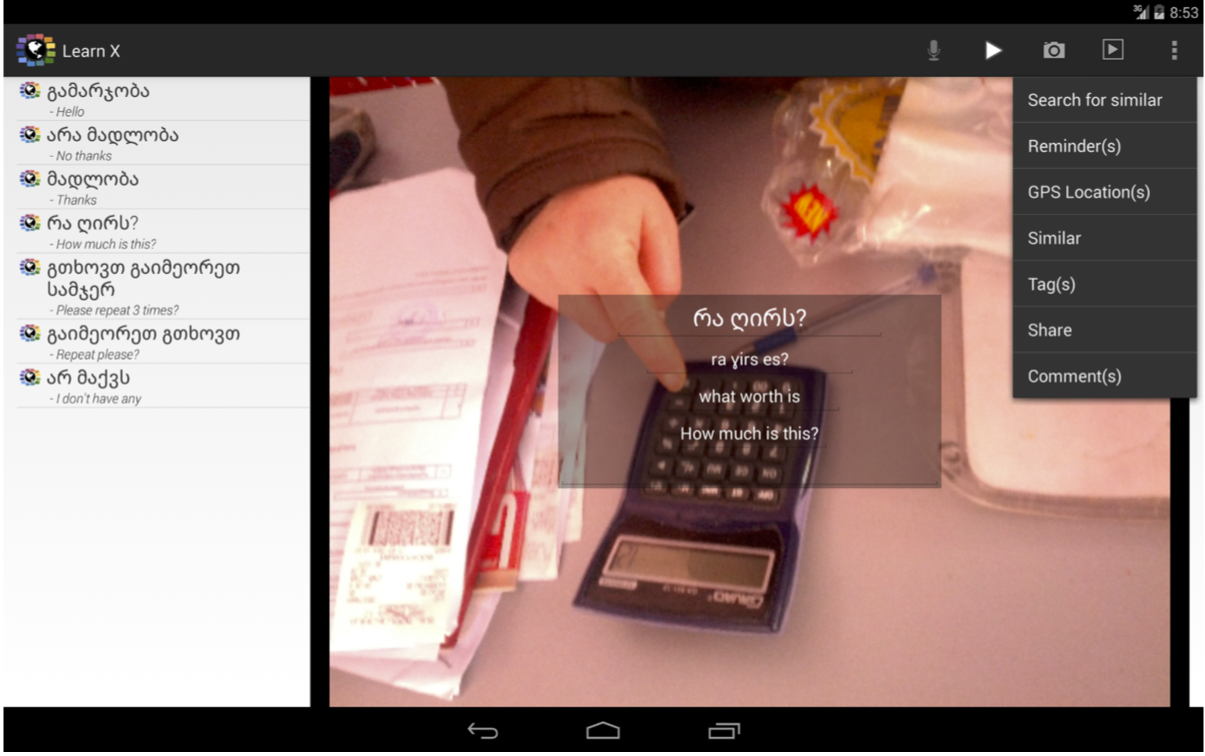
\includegraphics[width=3in]{figures/learnX}
\caption{Screenshot of Learn X, an Android app which lets users build language
learning apps using LingSync.}
\label{learn_x_screenshot}
\end{center}
\end{figure}

LingSync's permissions system was designed so that language community members
and heritage speakers of the language can use the multimedia data collection
features of Android phones (camera, audio, video) to construct their own
language learning lessons which are saved into their own corpus and/or
contributed to a team corpus.

Learn X is freely available for download%
\footnote{\url{https://play.google.com/store/apps/details?id=com.github.opensourcefieldlinguistics.fielddb.lessons.georgian}} %
as ``Georgian Together'' which we are field testing during the Spring 2014
semester with members of the \gls{tlg} volunteers.  Like heritage learners, TLG
volunteers spend their time surrounded with the language, can understand more
than they can speak, and what they speak about is highly dependent on what
their family speaks about most. LingSync's open-endedness and confidentiality
settings make it easy for teams to create and share vocabularies/phrases.
In fact, there are many social contexts which will not be acknowledged or
printed in any online grammar or second language materials, contexts which
users can elect to hide from other users, or share with certain users depending
on their comfort level.

In addition to language learning resources, communities may also benefit from
descriptive grammars, spell checkers, grammar checkers, autocorrect/predictive
typing, subtitling, translation memories, voice writing, content
creation/language representation on the web, and improved access to relevant
web search results. To facilitate access to content, we created a very simple
Georgian transliteration module which permits Georgian speakers to read
Georgian written in the Latin alphabet by (predominately) iPhone content
creators who do not have access to a Georgian keyboard, also freely available
for download.%
\footnote{\url{https://chrome.google.com/webstore/detail/kartuli-glasses/ccmledaklimnhjchkcgideafpglhejja}}


\subsection{Software Development for Low-resource Languages}\label{sec:software}

Many of the modules used to build LingSync can be integrated using HTML5 build tools in software for other purposes. All modules are registered on NPM as they stabalize. Readers are encouraged to consult \url{http://npmjs.org} for an up-to-date list.

\subsection{Computational Linguistics for Low-resource Languages}\label{sec:complinguistics}

Data collected by language documentation projects can also serve the language
community indirectly via the construction of computational tools and data sets
which can then help software developers build software which enables content in
low-resource languages, further facilitating the use of minority languages in
digital communication (both spoken and written). Thinking about these data uses
before and during data collection with speakers can help field teams think
about how to explaining the frequently abstract licensing language to
consultants via consent forms as well as potentially concretely identifying the
benefits  consultant's participation in the language resources effort has for
other members in the community. Language documentation projects can also
partner with Software Engineering or Computational Linguistics labs to
recompile corpora into gold standard data, and training data, or crowd source
annotations, build stemmers, and improve search and information retrieval. Many
of these results can be used to build more complex systems including
morphological analyzers, machine translation, text to speech systems, speech
recognition systems and in some cases such as Georgian even text summarization
for local law firms.

During the Spring 2014 semester we are training computer science masters
students at the Batumi Shota Rustaveli  State University in how to use
CMUSphinx tools to build speech recognition systems which can be delivered to
Android smart phone users. Initial pipelines have been prototyped using Bash
scripts but will not be in production as an Android app until after the
semester is concluded (June 2014). Corpus data are first through a
transliteration process to and then used to generate pronunciation dictionaries
which serve as input  to the open source Phonetisaurus Libraries
\cite{Novak:2012} for the generation of pronunciation entries of novel words.
The corpus data is extracted as raw text and used to generate n-gram language
models using the open source CMUCLMTK \cite{Clarkson:1997} language model
generation scripts which accept a pronunciation dictionary and sentence
delimited corpus as input. Acoustic models are adapted from existing acoustic
models via the export of utterance lines and corresponding audio and the 
\cite{Elmahdy:2010}. Finally, the language specific dictionary, language model,
and adapted acoustic model are provided to the PocketSphinx Android library to
produce n-best hypothesis for novel audio. While we expect that the result will
be poor for most small corpora in the system, automating the model training
pipelines can serve to increase interest in the process of speech recognition
among software developers from minority language populations  and also
encourage language communities to volunteer in the collection and annotation of
the sorts of data which are required to have more representative language
models and acoustic models \cite{Sarfraz:2010}.


\subsubsection{API}

For language documentation teams collaborating with Software Engineering labs
or Computational Linguistics labs LingSync web services expose a RESTful
\gls{api} for requests on resources.%
\footnote{RESTful means that combinations of \gls{url} patterns and HTTP methods
    names are mapped consistently and transparently to operations on the
    relevant resources. The payloads of all HTTP requests and responses are
\gls{json}}

\ref{fig:api-basic} illustrates the use of the LingSync \gls{api} for
authentication, the creation of an new record, and requesting all records.
\ref{fig:api-search} demonstrates use of the search \glspl{api}. Examples of
more sophisticated  \glspl{api} which provide specialized processing for
audio/video/image and text  are presented in \ref{sec:plugins}.

\begin{figure}[h]
\scriptsize

\begin{verbatim}
a) $ curl --cookie-jar my-cookies.txt\
  --request PUT\
  --header "Content-Type: application/json"\
  --data '{"username":"public", "password":"none"}'\
    https://api.lingsync.org/v2/users

b) $ curl --cookie my-cookies.txt\
  --request POST\
  --data '{"transcription": "omi imitaa"}'\
    https://api.lingsync.org/v2/corpora/public-curldemo

c) $ curl --cookie my-cookies.txt\
  --request GET\
    https://api.lingsync.org/v2/corpora/public-curldemo
\end{verbatim}
\caption{\texttt{curl} requests for authentication (a), creating a record (b)
and requesting all records (c)}
\normalsize
\label{fig:api-basic}
\end{figure}


\begin{figure}[h]
\scriptsize
\begin{verbatim}
a) $ curl --cookie my-cookies.txt\
  --request SEARCH\
  --data '{"query": {"filter": ["and", [
  ["data", "translations", "transcription", "=", "cat"],
  ["or", [["not", ["data", "transcription", "=", "*"]],
          ["data", "grammaticality", "=", null]]],
  ["data", "transcription", "regex", "^p"],
  ["data", "morpheme_gloss", "=", ""]]]}}'\
 https://api.lingsync.org/v2/corpora/public-curldemo
 
b) $ curl --cookie my-cookies.txt\
  --request SEARCH\
  --data '{"query": {"filter":
  ["data", "break_gloss_category", "regex",
    "-wa\|3SG\|Agr( |-|$)"]}}'\
 https://api.lingsync.org/v2/corpora/public-curldemo

c) $ curl --cookie my-cookies.txt\
  --request SEARCH\
  --data '{"tgrep2pattern": "/^[TI]P$/ < (DP << AP)"}'\
  https://api.lingsync.org/v2/corpora
\end{verbatim}
\caption{\texttt{curl} requests for complex search (a), unambiguous morpheme
search (b), TGrep2 structural search (c)}
\normalsize
\label{fig:api-search}
\end{figure}


\pagebreak

\appendix 

\section{LingSync Modules}

In this section we discuss in detail the timeline and budget for each of the modules that make up the LingSync application. The modules are grouped into core modules and dream modules which will be made when the budget becomes available. 

\label{sec:modules}
\subsection{Core Modules}

The project has three core modules which must be developed prior to additional modules. These are the {\it collaboration, corpus} and {\it lexicon} modules, briefly outlined in terms of functionality and timeline in the following sections.  Implementation of the three core modules began on April 20th 2012. The three core modules will be launched on August 1st at CAML in Patzun Guatemala. We estimate the three core modules and the software architecture to take 9.2 weeks to complete with three software developers,  and cost roughly \$23,800 before taxes. We will have its final time and costs on August 3rd 2012.


\newpage
\subsubsection{Collaboration Module}
The collaboration module shown in Table~\ref{table-collaboration}  deals with users, teams, permissions, user authentication,  as well as allowing users to see changes, modifications, and data verification in the form of an ``Activity Feed.'' An activity feed is a common design pattern which allows users to learn form other users how to use the software, what are popular functions other users are completing in addition to being a central location to update oneself on the activity in the corpus. The system will have special users called ``bot'' which are scripts or programs which power users can write in Javascript which will crawl their corpus and clean/automate batch actions.

We estimate the total cost of the collaboration module to be around \$5,700 before taxes. The implementation of the collaboration module was begun on April 20th 2012, and finished on August 1st 2012, with the exception of Team Feed and Team Preference Widgets. 
%User/Consultant/Team tests are not done either. 
\begin{table}[h]
\begin{center}
  \begin{tabular}{ | lcl | }
\hline
Iteration&	Hours&	Technology	\\
\hline
Software Architecture Design&	20&	Software Engineering	\\ 
Collaboration API on central server&	30&	Software Engineering\\ 
Users Model&	15&	Javascript	\\ 
consultant Model&	15&	Javascript	\\ 
Team Model&	15&	Javascript	\\ 
Bot Model&	15&	Javascript	\\ 
User Activity Model&	8&	Javascript	\\ 
Team Feed Widget&	25&	HTML5	\\ 
User list item Widget&	16&	HTML5	\\ 
Team Preferences Widget&	8&	HTML5	\\ 
User Profile Widget&	8&	HTML5	\\ 
User Tests&	30&	Javascript \\ 
Consultant Tests&	30&	Javascript	\\ 
Team Tests&	30&	Javascript	\\ 
Android Deployment&	15&	Java	\\ 
Chrome Extension Deployment&	20&	Javascript \\ 
Heroku Deployment&	5&	Integration	\\ 
%\# of weeks with 3 full time personnel&	2.5416666667& \\ 
\hline
  \end{tabular}
  \caption{The Collaboration Module is used to permit collaboration with teams and users. }
\label{table-collaboration}
  \end{center}
\end{table}


\newpage
\subsubsection{Corpus Module}
The corpus module shown in Table~\ref{table-corpus} deals with storing confidential data in the AES US Federal encryption standard, replicating the corpus locally on the  users' computers, as well as on a central server hosted either in the cloud, or on a linguistic department's server. The corpus module contains all of the core logic, including data fields, session fields, as well as data lists which are used to curate lists of data for handouts or publication either in linguistic articles or as web widgets embedded in external websites such as linguistic department blogs, or project pages. The corpus module is also where search of datum is implemented. 

We estimate the total cost of the corpus module to be around \$9,200 before taxes. The implementation of the corpus module was begun on April 20th 2012, and finished on August 1st 2012, with the exception of Corpus diff Widget.
\begin{table}[htbp]
\begin{center}
  \begin{tabular}{ | lcl | }
\hline

Iteration&	Hours&	Technology	\\
\hline
Software Architecture Design&	20&	Software Engineering	\\ 
Corpus API on corpus server&	20&	Software Engineering\\ 
Corpus Model&	8&	Javascript	\\ 
Session Model&	8&	Javascript	\\ 
Datum Model&	8&	Javascript	\\ 
Datum status model&	8&	Javascript	\\ 
DataList Model&	8&	Javascript	\\ 
Confidential datum encrypter&	16&	Javascript	\\ 
Audio upload and play logic&	8&	Javascript	\\ 
Corpus DB  implementation on Android&	20&	Java	\\ 
Corpus DB  implementation on Chrome&	20&	Javascript	\\ 
Corpus DB  implementation on Node.js&	20&	Javascript \\ 
Corpus versioning Logic&	25&	Javascript	\\ 
Corpus Preferences Widget&	6&	HTML5	\\ 
Session Preferences Widget&	6&	HTML5	\\ 
Datum Preferences Widget&	20&	HTML5 \\ 
Datum Status Preferences Widget&	16&	HTML5	\\ 
DataList Preferences Widget&	6&  HTML5 \\ 
Corpus sync logic&	10&  Javascript \\ 
Corpus diff Widget (to show before sync)&	10&  HTML5 \\ 
Insert Unicode Character Widget&	10&  HTML5 \\ 
Corpus Details Widget&	6&  HTML5 \\
Session Details Widget&	6&  HTML5 \\  
Datum Details Widget&	20&  Javascript \\ 
DataList Widget&	30&  Javascript \\ 
Global Search logic&	30&  Javascript \\ 
Power Search logic&	80&  Javascript \\ 
Corpus Tests&	5&  Javascript \\ 
Session Tests&	10&  Javascript \\ 
Datum Tests&	10&  Javascript \\ 
Datum Status Tests&	10&  Javascript \\ 
DataList Tests&	20&  Javascript \\ 
Heroku Deployment&	5&  Integration \\ 
\hline
  \end{tabular}
 \caption{The Corpus Module is used to sync, share, edit, tag, categorize and open data. }
\label{table-corpus}
  \end{center}
\end{table}
%# of weeks with 3 full time personnel	4.20833333333333


\newpage
\subsubsection{Lexicon Module}

The lexicon module show in Table~\ref{table-lexicon} is used for search. It is loosely modeled after a mental lexicon, in a network of morphemes, allomorphs, orthographie(s), glosses and translations.  It is not a dictionary but rather a connected graph similar to theoretical models of mental lexicons (for a dictionary see the Dictionary Module in \S~\ref{module-dictionary}). As a connected graph it is the most useful structure to index datum and search for datum real time while data entry is happening. 
%One requested use-case was to have the search open for a particular morpheme/category and have datum which are entered show up in the search results. 

We estimate the total cost of the lexicon module to be around \$7,300 before taxes. The implementation of the lexicon module was begun on April 20th 2012. We will know its final costs on August 3rd 2012.

\begin{table}[htbp]
\begin{center}
  \begin{tabular}{ | lcl | }
\hline

Iteration&	Hours&	Technology	\\
\hline
Software Architecture Design&	20&	Software Engineering	\\ 
Lexicon API on Lexicon server&	20&	Software Engineering\\ 
Lexicon Model&	6&	Javascript	\\ 
Morpheme Model&	6&	Javascript	\\ 
Allomorph Model&	6&	Javascript	\\ 
Gloss Model&	6&	Javascript	\\ 
Orthography Model&	16&	Javascript	\\ 
Lexicon DB  implementation on Android&	20&	Java	\\ 
Lexicon DB  implementation on Chrome&	20&	Javascript	\\ 
Lexicon DB  implementation on Node.js&	20&	Javascript \\ 
Lexicon versioning Logic&	10&	Javascript	\\ 
Lexicon Preferences Widget&	6&	HTML5	\\ 
Morpheme Tests&	6&	Javascript	\\ 
Allomorph Tests&	6&	Javascript \\ 
Gloss Tests&	6&	Javascript	\\ 
Orthography Tests&	8&  Javascript \\ 
Lexicon Analysis Widget&	10&  HTML5 \\ 
Lexicon sync logic&	10&  Javascript \\ 
Lexicon diff Widget (to show before sync)&	10&  HTML5 \\ 
Lexicon Details Widget&	6&  HTML5 \\
Lexicon Tests&	12&  Javascript \\  
Heroku Deployment&	5&  Integration \\ 
\hline
  \end{tabular}
 \caption{The Lexicon Module is used to house, and read lexicon entries to be used for the glosser.}
 \label{table-lexicon}
  \end{center}
  

\end{table}
%# of weeks with 3 full time personnel	1.95833333333333

\subsection{``Dream'' Modules}

The "dream" modules allow for more features that will save researchers time in their data entry and data analysis, but which are not necessary for simply entering and transcribing data. These modules are on hold until budget becomes available.


\subsubsection{Language Learning Module}
The language learning module shown in Table ~\ref{tab:langlearn} enables researchers and language teachers to create language learning aids from the data in existing corpora and from the data newly collected for the purpose of language learning. The learning aids aim to help language learners improve their listening and speaking skills. The orthographic lines (i.e. utterance and morpheme lines) and the attached audio or video recordings of a datum are taken as materials to create a lesson. 


The prototype of the language learning module was begun on September 13th 2012.

\begin{table}[htbp]
\begin{center}
  \begin{tabular}{ | lcl | }
\hline
Iteration &	 Hours &	Technology	\\
\hline
-- Prototype && \\ 
Software Architecture Design & 55 & Software Engineering \\
Lesson Datum Model & 15  & Javascript \\
Lesson Datum Listen and Repeat View & 20  & Javascript \\
XML import logic  & 6 & Javascript \\ 
Datum to Lesson logic  & 6  & Map Reduce \\ 
DataList to Unit logic  & 6  & Map Reduce \\ 
Corpus to Language Learning logic  &  10  & Map Reduce \\ 
Main Manu Dashboard  & 6  & HTML \\ 
Student LIsten and Repeat Dashboard  & 10  & HTML \\ 
Student Instructions View  & 6  & Javascript \\ 
Audio Visualization View  & 30  & Javascript \\ 
Audio Play/Record View  & 10  & Javascript \\ 
Audio Text Time Alignment logic  & 20  & Javascript \\ 
Audio Record Android logic  &  6  & Java \\ 
Android Packaging  & 15  & Java \\ 
% # of weeks with 1 full-time personnel supervising 2 interns 4.775 
\hline 
Software Architecture Design & 40 & Software Engineering  \\ 
Teacher User Model  &  10 &  Javascript \\ 
Teacher User View  &  40  & Javascript \\ 
Language Learning Corpus  &  10 &  Javascript \\ 
Language Learning Corpus View  &  40  & Javascript \\ 
Language Learning Corpus Dashboard  &  10  & HTML \\ 
Student User Model  &  30  & Javascript \\ 
Student User View  &  60  & Javascript \\ 
Datum Shadowing Lesson Model  & 10 & Javascript \\ 
Datum Shadowing Lesson View  &  10  &  Javascript \\ 
Student Shadowing Lesson Dashboard &  40 & HTML \\ 
Datum Quiz Multiple Choice Model  & 20  & Javascript \\ 
Datum Quiz Multiple Choice View  &  20  & Javascript \\ 
Student Quiz Dashboard  & 120  & HTML \\ 
Datum Prompted Production Model  & 20  & Javascript \\ 
Datum Prompted Production View  & 20  & Javascript \\ 
Student Prompted Productions Dashboard  &  40  & HTML \\ 
Feedback Comment Model  & 10  & Javascript \\ 
Feedback Comment View  & 40  & Javascript \\ 
Comment Teacher Feedback logic & 6  & Map Reduce \\ 
Audio import to Multiple Utterances logic   & 60  & Praat \& Javascript \\ 
Audio File Server  & 140  & Node \\ 
% # of weeks with 1 full-time personnel 19.4 
\hline
  \end{tabular}
 \caption{The Language Learning Module enables to use data in the database to create lessons for language learners.  }
  \label{tab:langlearn}
  \end{center}
\end{table}



\subsubsection{Phonological Search Module}
The phonological search module shown in Table~\ref{tab:phono} is used to search for phonological features in context. It consists of a phonology ontology (a general purpose feature geometry/articulatory feature ontology, or a customized ontology created by the users for their language of interest) which lets the user search for potential minimal pairs or phonological features in context to verify with consultants or to prepare psycholinguistic experiments. The phonological search module is used by the {\it  phonetic aligner} module to generate a ``dictionary.txt'' file containing orthography and phones which is used by the phonetic aligner module.

We estimate the cost of the phonological search module to be roughly \$2,200 before taxes. The Phonological search, or the phonetic aligner module is currently schedule to begin in September 2012, we haven't yet decided which is a priority.

\begin{table}[htbp]
\begin{center}
  \begin{tabular}{ | lcl | }
\hline
Iteration&	Hours&	Technology	\\
\hline
Phonology Ontology for phonological search&	60&	Java	\\ 
Lexicon Visualization Widget&	40&	Javascript	\\ 
Lexicon Editing Widget&	20&	Javascript	\\ 
\hline
  \end{tabular}
 \caption{This module is a subportion of the Lexicon Module.}
  \label{tab:phono}
  \end{center}
\end{table}
%# of weeks with 1 full time personnel	3


\newpage
\subsubsection{Phonetic Aligner Module}
The phonetic aligner module show in Table~\ref{tab:aligner} makes it possible to use attached audio recordings and the orthographic/utterance lines of datum to create a dictionary unique to the corpus' language, and to run the ProsodyLab Aligner, a machine learning algorithm which uses Hidden Markov Models to predict boundaries between phones and creates a Praat TextGrid with estimated phone boundaries, saving hours of boundary tagging. We also have factored in a bit of sound editing to facilitate the process of creating audio files which correspond closely to the utterance line in the datum's fields. 


We estimate the cost of the phonetic aligner module to be roughly \$9,800 before taxes. The phonetic aligner or the phonological search module is currently scheduled to begin in September 2012, we haven't yet decided which is a priority.
\begin{table}[htbp]
\begin{center}
  \begin{tabular}{ | lcl | }
\hline

Iteration&	Hours&	Technology	\\
\hline
Software Architecture Design&	10&	Software Engineering	\\ 
Aligner API on Lexicon server&	10&	Software Engineering\\ 
Dictionary Model&	15&	Javascript	\\ 
Aligner DB implementation&	80&	Integration	\\ 
Aligner Machine Learning Integration&	80&	Java	\\ 
Aligner Preferences Widget&	8&	HTML5	\\ 
Audio Waveform Visualization logic&	30&	Javascript	\\ 
Audio Spectrogram Visualization logic&	?&	Javascript \\ 
Transcription User Interface&	80&	HTML5	\\ 
TextGrid export&	20&  Javascript \\ 
Dialect Profile Widget&	         8&  HTML5 \\ 
Orthography Tests&	30&  Javascript \\ 
Training Tests&	30&	Java	\\ 
Heroku Deployment&	5&  Integration \\ 
\hline
  \end{tabular}
  \caption{The Aligner Module is used to create TextGrids from the orthography and the audio files, used for prosody and phonetic analysis.}
  \label{tab:aligner}
  \end{center}
\end{table}
%# of weeks with 1 full time personnel	10.15



\newpage
\subsubsection{Dictionary Module}

The dictionary module shown in Table~\ref{tab:dictionary}is used to crawl the corpus to gather citations and examples to build a Wiktionary dictionary for the corpus' language, as required by some grants which focus on endangered/minority languages. The dictionary module is quite complex and the central component of many online fieldlinguistics databases. 	

We estimate the dictionary module to cost roughly \$ 18,800 before taxes. The dictionary module is not currently scheduled until we have more users who require its functionality.
\label{module-dictionary}
\begin{table}[htbp]
\begin{center}
  \begin{tabular}{ | lcl | }
\hline

Iteration&	Hours&	Technology	\\
\hline
Software Architecture Design&	40&	Software Engineering	\\ 
Dictionary API on Lexicon server&	30&	Software Engineering\\ 
Semantic Model&	60&	Javascript	\\ 
Syntactic Model&	60&	Javascript	\\ 
Citation Model&	60&	Javascript	\\ 
Synonyms Model&	60&	Javascript	\\ 
Dictionary DB implementation&	80&	Integration	\\ 
Dictionary Training Logic&	80&	Java	\\ 
Web Spider Training Logic&	100&	Java	\\ 
Dictionary Preferences Widget&	8&	HTML5	\\ 
Dictionary WordNet Analysis Widget&	120&	HTML6	\\ 
Dialect Profile Widget&	8&	HTML5 \\ 
Semantic Tests&	30&	Javascript	\\ 
Syntactic Tests&	30&  Javascript \\ 
Citation Tests&	         30&  Javascript \\ 
Synonyms Tests&	30&  Javascript \\ 
Spider Tests&	30&	Java \\ 
Training Tests&	30&	Java	\\ 
Heroku Deployment&	5&  Integration \\ 
\hline
  \end{tabular}
 \caption{The Dictionary Module is used to share the lexicon in the form of a WordNet/Wiktionary dictionary with the language community as required by some grants.}
  \label{tab:dictionary}
  \end{center}
\end{table}
%# of weeks with 1 full time personnel	22.275


\newpage
\subsubsection{Glosser Module}
The glosser module show in Table~\ref{tab:glosser} is designed to make the app ``smarter'' and to reduce the amount of time spent entering predictable information such as glosses. The glosser can use any existing morphological analysis tool to break down the utterance/orthography line  into a probable morphological segmentation using known morphemes in the lexicon, and enters a probable gloss for the morphemes in the glossing line. The glosser module is designed to reduce redundant data entry, not to provide accurate glosses. It is of course crucial that predicted morpheme segmentation and glosses be corrected by users, particularly in languages where morphemes are ambiguous, or where morphemes are short and hence there are more ambiguous morpheme segmentations for words. 


We estimate the glosser module to cost roughly \$17,800. The glosser module is not currently scheduled until we have more users who require its functionality.
\begin{table}[htbp]
\begin{center}
  \begin{tabular}{ | lcl | }
\hline

Iteration&	Hours&	Technology	\\
\hline
Software Architecture Design&	40&	Software Engineering	\\ 
Glosser API on Lexicon server&	30&	Software Engineering\\ 
Morpheme Model&	15&	Javascript	\\ 
Allomorph Model&	15&	Javascript	\\ 
Gloss Model&	15&	Javascript	\\ 
Orthography Model&	30&	Javascript	\\ 
Glosser DB implementation&	80&	Integration	\\ 
Glosser Prediction Logic&	80&	Java	\\ 
Glosser Machine Learning Logic&	80&	Java	\\ 
Glosser Training Logic&	80&	Java	\\ 
Web Spider Training Logic&	80&	Java	\\ 
Glosser Preferences Widget&	8&	HTML5	\\ 
Morphological Analysis Widget&	40&	HTML6	\\ 
Dialect Profile Widget&	8&	HTML5 \\ 
Morpheme Tests&	30&	Javascript	\\ 
Allomorph Tests&	30&  Javascript \\ 
Gloss Tests&	         30&  Javascript \\ 
Orthography Tests&	30&  Javascript \\ 
Spider Tests&	30&	Java \\ 
Training Tests&	30&	Java	\\ 
Heroku Deployment&	5&  Integration \\ 
\hline
  \end{tabular}
   \caption{The Glosser Module is used to automatically gloss datum, smarter than the standard lexicon.}
  \label{tab:glosser}
  \end{center}
\end{table}
%# of weeks with 1 full time personnel	19.65

\subsubsection{Web Spider Module}

The Web Spider module shown in Table~\ref{table-spider} is a non-crucial module which allows researchers with limited access to consultants to gather data using blogs or forums. The web spider also provides an additional source of context to assist consultants in providing grammaticality judgements, as well as additional contexts where morphemes appear. For example, ``ke'' is largely considered a postposition by Urdu-consultants with explicit knowledge, however it is often produced as other functional morphemes in everyday spoken contexts. Blog/forum data can be used to discover these additional contexts.


The Web Spider module is currently not a scheduled module.  It will not become a priority until we have more users who require its functionality.

\begin{table}[htbp]

\begin{center}
  \begin{tabular}{ | lcl | }
\hline
Iteration&	Hours&	Technology	\\
\hline
Corpus Visualization Widget&	40&	HTML5	\\ 
Web Spider Training Logic&	60&	Java	\\ 
\hline
  \end{tabular}
  \caption{The Spider module allows for collection and annotation of E-Language data.}
\label{table-spider}
  \end{center}
\end{table}
%# of weeks with 1 full time personnel	2.5



\newpage
\subsubsection{User Support \& Maintenance}

The user support  \& maintenance module shown in Table~\ref{tab:support} includes general support, new features, upgrades, and maintenance. User support includes answering user's emails, helping system administrators install the app and its various server apps on their department server, creating video tutorials, screen casts and sample data to help users figure out the application and begin using it immediately, as well as discover some of its advanced/unexpected features. 

We estimate the user support \& maintenance module to cost roughly \$30,200 if we include unlimited support, or \$13,000 if we do not include email and tech support but only new features, maintenance, video tutorials and user guides.

\footnotesize
\begin{table}[htbp]
\begin{center}
  \begin{tabular}{ | lcl | }
\hline  

Iteration&	Hours&	Technology	\\
\hline
Sample data&	30&	Linguistics	\\ 
Integrate software with sample data&	30&	Javascript\\ 
Screencasts on how to use the app(s)&	24&	Quicktime/YouTube	\\ 
Screencasts on how to modify the code&	40&	Quicktime/YouTube	\\ 
Server maintenance&	20&	Integration	\\ 
Monitor server costs and develop pricing plan&	100&   Business	\\ 
Answer user emails&	250&	Support	\\ 
Read twitter feeds and facebook channels&	100&	Support \\ 
Help IT/developers install and set up  & &\\ 
the server on their department servers&	50&	Support	\\ 
Upgrade javascript/android libraries&	40&  Javascript \\ 
Amazon EC2 server CPU+Memory+Bandwidth&	         &  Server \\ 
Release new versions&	160&  Javascript \\ 
\hline
  \end{tabular}
 \caption{User Support includes 1 year of product support and project growth. It is needed to make a longterm viable and useful tool that field linguists can adopt for their labs or for their field methods courses.} 
  \label{tab:support}
  \end{center}
\end{table}
%# of weeks with 1 full time personnel	21.1







\bibliography{ComputEL/bibliography}






\end{document}


